\documentclass[10pt,leqno]{amsart}
\usepackage{graphicx}
\baselineskip=16pt

\usepackage{indentfirst,csquotes}
\usepackage{here}

\topmargin= .5cm
\textheight= 20cm
\textwidth= 32cc
\baselineskip=16pt

\evensidemargin= .9cm
\oddsidemargin= .9cm

\usepackage{amssymb,amsthm,amsmath}
\usepackage{xcolor,paralist,hyperref,fancyhdr,etoolbox}
\newtheorem{theorem}{Theorem}[]
\newtheorem{definition}[theorem]{Definition}
\newtheorem{example}[theorem]{Example}
\newtheorem{lemma}[theorem]{Lemma}
\newtheorem{proposition}[theorem]{Proposition}
\newtheorem{corollary}[theorem]{Corollary}
\newtheorem{conjecture}[theorem]{Conjecture}

% \titleformat{\section}[display]{\normalfont\huge\bfseries\centering}{\centering\chaptertitlename\thechapter}{10pt}{\Large}
% \titlespacing*{\section}{0pt}{0ex}{0ex}

\hypersetup{ colorlinks=true, linkcolor=black, filecolor=black, urlcolor=black }
\def\proof{\noindent {\it Proof. $\, $}}
\def\endproof{\hfill $\Box$ \vskip 5 pt }
\setcounter{section}{-1}

\usepackage{lipsum}

% \begin{document}
% \title{A3 (HEP) Coursework Theory Report} %%%%%%%%%%%%
% \author[Initial Surname]{Baiyuan Chen}
% \date{}
% % \address{Address}
% \email{chenbaiyuan75@gmail.com}

% % \begin{abstract}
% % Abstract 
% % \end{abstract}

% \maketitle

% \section{Introduction}

\begin{document}

\begin{titlepage}
\centering
\vspace*{2cm}

{\LARGE \bfseries A3 High Energy Physics Coursework Theory Report\par}

\vspace{1.5cm}

{\large Baiyuan Chen\par}
\vspace{0.3cm}
{\large CRSID: bc654\par}
\vspace{0.3cm}
{\large bc654@cam.ac.uk\par}

\vspace{1.5cm}

{\large Word Count: $\sim$1605\par}

\vspace{1.5cm}

{\large MPhil in Data Intensive Science\par}
\vspace{0.3cm}
{\large University of Cambridge\par}
% \vspace{0.3cm}
% {\large \today\par}
\vspace{1.5cm}

{\small\textit{Below, ``we'' is used instead of ``I'' to follow the convention of scientific writing.}\par}

\vfill
\end{titlepage}

\setcounter{section}{-1}
\section{Introduction}

Symmetries are central to modern physics. Lorentz invariance underpins
special relativity, while local gauge symmetries such as $\mathrm{SU}(2)$
govern the structure of the electroweak interaction. When neural networks 
are used to represent physical fields, a generic architecture does not 
automatically respect these symmetries and can only learn them approximately 
from data. Following the coursework, this report studies two pre-trained networks,
NN1 and NN2, that approximate an $\mathrm{SU}(2)$ scalar doublet and a
gauge--boson field respectively. We first verify their transformation
properties analytically and numerically (Sections~1--2), then construct
alternative architectures in which equivariance is enforced exactly by
restricting the network input to Lorentz invariants (Section~3). Finally,
we build a classical Lagrangian from these equivariant fields and confirm
its invariance under both Lorentz and $\mathrm{SU}(2)$ transformations
(Section~4).

\section{Q1: Equivariance of NN1: SU(2) Fundamental and Lorentz Scalar}

NN1 is a generic fully connected network ($4 \to 128 \to 128 \to 128 \to 4$
with ReLU activations) that maps spacetime coordinates
$x = (t,x,y,z) \in \mathbb{R}^4$ to four real outputs, which we package
as a complex SU(2) doublet
$\Phi = (\phi_1 + i\phi_2,\; \phi_3 + i\phi_4)^T \in \mathbb{C}^2$.
Four real outputs map naturally to two complex components, matching the
dimensionality of the fundamental representation of SU(2).

\textbf{Lorentz scalar (analytical).}
A scalar field satisfies $\Phi(\Lambda x) = \Phi(x)$ for all Lorentz
transformations $\Lambda \in \mathrm{SO}(3,1)$. This is a non-trivial
constraint: a generic MLP takes all four components of $x$ as independent
inputs and could learn functions that are \emph{not} Lorentz-invariant.
For the scalar condition to hold, the network must effectively depend only
on Lorentz-invariant input combinations, the simplest being
$x_\mu x^\mu = t^2 - x^2 - y^2 - z^2$. Since NN1 has no architectural
mechanism enforcing this (unlike the equivariant network in Section~3),
the scalar property can only be approximate, arising from how the weights
were tuned.

\textbf{Lorentz scalar (numerical).}
We evaluate NN1 at 500 random points in $[-3, 3]^4$ and compute the
relative error
$\varepsilon = \|\Phi(\Lambda x) - \Phi(x)\| / \|\Phi(x)\|$ under 50
random transformations. Rotations are generated from a random axis
(normalised Gaussian) and uniform angle in $[0, 2\pi]$; boosts use a
random rapidity in $[0, 0.8]$ along a random direction. We restrict to
transformed points within the training domain $|x_i| \leq 5$ and filter
for $\|\Phi\| > 0.1$ to avoid inflated relative errors from near-zero
outputs. The mean relative errors are approximately 5.6\% for rotations
and 4.2\% for boosts, with maximum errors of approximately 6.6\% in both
cases, confirming that NN1 is an approximate Lorentz scalar.

\textbf{SU(2) fundamental (analytical).}
The fundamental (spin-$\tfrac{1}{2}$) representation of SU(2) consists of
$2 \times 2$ unitary matrices with unit determinant acting on vectors in
$\mathbb{C}^2$. Under a global transformation $U \in \mathrm{SU}(2)$ the
doublet transforms as $\Phi \to U\Phi$, which is the defining
property of the fundamental representation. Crucially, SU(2) is an internal
symmetry: it acts only on the field components (the output space) and not
on the spacetime coordinates (the input), so the doublet structure is a
consequence of how we package the four real outputs into $\mathbb{C}^2$
and places no constraint on the network weights. Unitarity
($U^\dagger U = I$) guarantees that $\Phi^\dagger\Phi$ is preserved, and
the generators $\tau_a = \sigma_a / 2$ (with $\sigma_a$ the Pauli
matrices) satisfy the SU(2) algebra
$[\tau_a, \tau_b] = i\epsilon_{abc}\,\tau_c$.

\textbf{SU(2) fundamental (numerical).}
Since SU(2) is internal, the transformation $\Phi \to U\Phi$ acts on the
output and does not involve the network, so any equivariance test reduces
to a check of the representation theory. We verify consistency by
evaluating NN1 at sample points, applying random $U \in \mathrm{SU}(2)$,
and confirming $\Phi^\dagger\Phi = (U\Phi)^\dagger(U\Phi)$. Differences
are of order $10^{-9}$ (Table~\ref{tab:q1_su2}), consistent with float32
precision. This test confirms unitarity of $U$ rather than a learned
property of the network, which is expected: for an internal symmetry the
equivariance is \emph{exact by construction} once the output is packaged
as a doublet.

\begin{table}[h]
    \centering
    \caption{SU(2) unitarity check for NN1: $|\Phi^\dagger\Phi - (U\Phi)^\dagger(U\Phi)|$
    under random $U \in \mathrm{SU}(2)$.}
    \label{tab:q1_su2}
    \begin{tabular}{cccc}
    Point & $|\Phi|^2$ before & $|\Phi|^2$ after $U$ & $|\Delta(\Phi^\dagger\Phi)|$ \\
    \hline
    0 & 1.028494 & 1.028494 & 9.01e-10 \\
    1 & 0.968938 & 0.968938 & 3.45e-08 \\
    2 & 0.071719 & 0.071719 & 1.66e-09 \\
    3 & 0.786423 & 0.786423 & 1.66e-09 \\
    4 & 0.815356 & 0.815356 & 1.73e-08
    \end{tabular}
\end{table}

\section{Q2: Equivariance of NN2: SU(2) Adjoint and Spin-1}

NN2 is a generic MLP with the same architecture as NN1 but with 12 outputs,
which we reshape into a $4 \times 3$ matrix $W_\mu^{\,a}(x)$ where
$\mu = 0,1,2,3$ is the Lorentz index and $a = 1,2,3$ is the SU(2)
adjoint index (matching $\dim\,\mathrm{SU}(2) = 3$).

\textbf{Lorentz spin-1 (analytical).}
A Lorentz vector (spin-1) field transforms as
$W_\mu^{\,a}(\Lambda x) = \Lambda_\mu^{\ \nu}\,W_\nu^{\,a}(x)$:
the $4 \times 4$ Lorentz matrix acts on the spacetime index $\mu$ while
the internal index $a$ is left untouched. As with NN1, the generic MLP
architecture has no mechanism enforcing this equivariance, so it can only
hold approximately.

\textbf{Lorentz spin-1 (numerical).}
Using the same testing protocol as Section~1 (500 points, 50
transformations, $\|W\| > 0.1$ filter), we compute
$\varepsilon = \|W_\mu^a(\Lambda x) - \Lambda_\mu^{\ \nu} W_\nu^a(x)\|
/ \|W(x)\|$. The mean relative errors are approximately 23\% for
rotations and 14\% for boosts, with maximum errors of approximately
28\% and 27\% respectively, which are substantially larger than NN1 and indicates
a coarser approximation. 
The error grows monotonically with the
transformation angle (Figure~\ref{fig:q2_angle}). This is expected for
a network trained to approximate equivariance: any smooth map can be
expanded as $W_\mu^a(\Lambda x) = \Lambda_\mu^{\ \nu} W_\nu^a(x) +
\delta W_\mu^a(x, \Lambda)$, where the violation $\delta W$ vanishes at
$\Lambda = I$ and grows with the size of the transformation. For a
rotation by angle $\theta$, $\Lambda = I + \theta\,K + \mathcal{O}(\theta^2)$
where $K$ is the generator, so the leading violation is
$\mathcal{O}(\theta)$, consistent with the approximately linear growth
seen at small angles in Figure~\ref{fig:q2_angle}.

\begin{figure}[htbp]
    \centering
    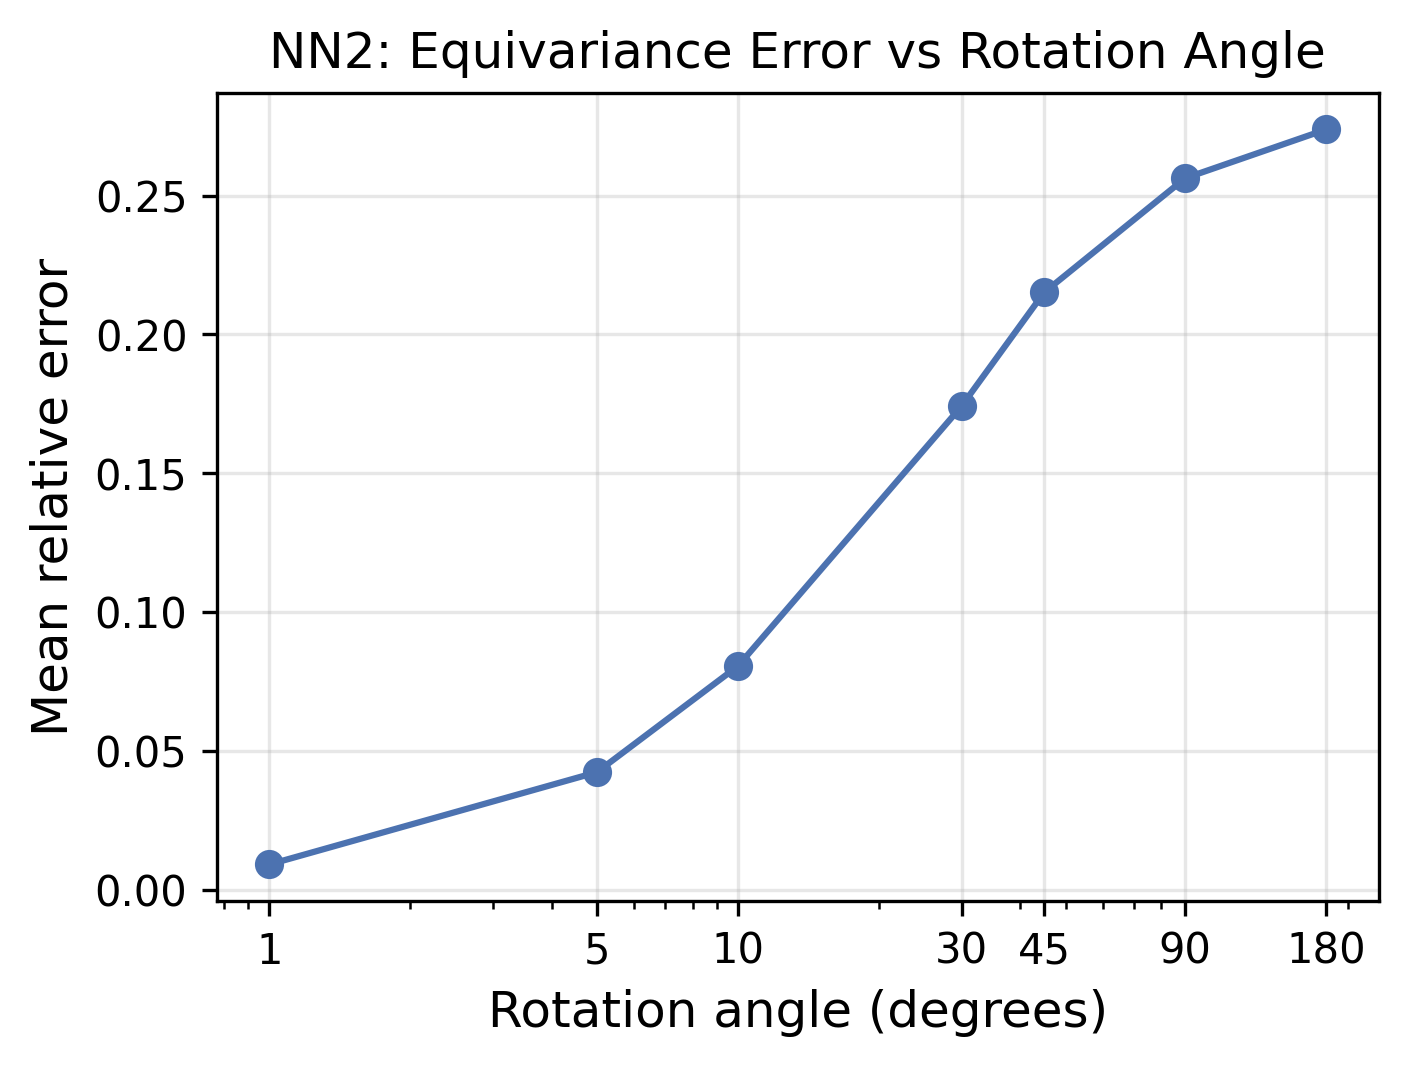
\includegraphics[width=0.4\textwidth]{../figures/thy_q2_angle.png}
    \caption{Relative error in $W_\mu^{\,a}(\Lambda x)$ vs transformation angle.}
    \label{fig:q2_angle}
\end{figure}

\textbf{SU(2) adjoint (analytical).}
The adjoint representation of SU(2) acts on the three-dimensional space
of the Lie algebra (spanned by the Pauli matrices $\sigma^a$). Under a
global $U \in \mathrm{SU}(2)$ the representation matrix is a real
$3 \times 3$ rotation
$R^{ab} = \tfrac{1}{2}\,\mathrm{Tr}(\sigma^a\, U\, \sigma^b\, U^\dagger)$,
and the field transforms as $W_\mu^{\,a} \to R^{ab}\,W_\mu^{\,b}$. As
with Q1, SU(2) is internal and does not act on the coordinates, so this
transformation law follows from identifying the index $a$ with the Lie
algebra basis. The matrix $R$ is automatically a proper rotation
($\det R = 1$, $RR^T = I$), so the adjoint invariant
$W_\mu^{\,a}\,W^{\mu\,a}$ is preserved.

\textbf{SU(2) adjoint (numerical).}
As in Section~1, the SU(2) transformation is internal and acts only on
the output, so the test reduces to verifying the representation theory.
We confirm that the computed $R$ matrices are proper rotations
($\det R = 1$, $\|RR^T - I\| \sim 10^{-15}$) and that the adjoint
invariant $W_\mu^{\,a}\,W^{\mu\,a}$ is unchanged under random
$R \in \mathrm{SO}(3)$. Differences are of order $10^{-8}$
(Table~\ref{tab:q2_su2}), consistent with machine precision and
confirming that the adjoint structure is exact by construction once the
index $a$ is identified with the Lie algebra basis.

\begin{table}[H]
\centering
\caption{SU(2) adjoint invariance check for NN2: $W_\mu^a W^{\mu a}$ before and after adjoint rotation $R$.}
\label{tab:q2_su2}
\begin{tabular}{cccc}
Point & $W_\mu^{\,a}W^{\mu\,a}$ before & after $R$ & $|\Delta|$ \\
\hline
0 & 0.037461 & 0.037461 & 9.03e-10 \\
1 & 2.396670 & 2.396670 & 4.13e-07 \\
2 & 0.407864 & 0.407864 & 1.52e-08 \\
3 & 2.395378 & 2.395378 & 4.02e-08 \\
4 & 0.848923 & 0.848923 & 4.31e-08
\end{tabular}
\end{table}

\section{Q3: Construction and Training of Equivariant Networks}

Rather than relying on weight tuning to learn symmetries approximately,
we build them into the architecture so they hold exactly.

\subsection*{Analytical form}
\mbox{}\\
We construct equivariant models of NN1 and NN2, denoted
EquivariantPhi and EquivariantW, respectively.

\textbf{EquivariantPhi.}
The only Lorentz-invariant scalar that can be formed from a single
spacetime point is $s = x_\mu x^\mu = t^2 - x^2 - y^2 - z^2$. We
therefore define
\begin{equation}\label{eq:eq_phi}
\Phi(x) = \mathrm{MLP}(s) \in \mathbb{R}^4.
\end{equation}
Since $s$ is invariant under Lorentz transformations,
$\Phi(\Lambda x) = \mathrm{MLP}(s(\Lambda x)) = \mathrm{MLP}(s(x))
= \Phi(x)$ by construction. The four real outputs are packaged as an
SU(2) doublet exactly as in Section~1.

\textbf{EquivariantW.}
The only Lorentz 4-vector available from a single point is $x_\mu$ itself.
The most general equivariant ansatz is therefore
\begin{equation}\label{eq:eq_W}
W_\mu^{\,a}(x) = f^a(s)\,x_\mu,
\end{equation}
where $f^a(s)$ is an MLP mapping $s \to \mathbb{R}^3$ (three adjoint
components). Under a Lorentz transformation,
$W_\mu^{\,a}(\Lambda x) = f^a(s)\,(\Lambda x)_\mu
= \Lambda_\mu^{\ \nu}\,f^a(s)\,x_\nu
= \Lambda_\mu^{\ \nu}\,W_\nu^{\,a}(x)$,
which is the correct spin-1 transformation law, holding exactly by
construction. The SU(2) adjoint structure is inherited from the index $a$
as in Section~2.

\subsection*{Implementation and results}
\mbox{}\\
Both MLPs use three hidden layers of 128 units with ReLU activations. We generate
training data by evaluating NN1/NN2 on 30{,}000 random points in
$[-5, 5]^4$ (5{,}000 for validation) and train with Adam ($\mathrm{lr}
= 10^{-3}$) and ReduceLROnPlateau for 150 epochs
(Figure~\ref{fig:q3_training}).

\begin{figure}[htbp]
    \centering
    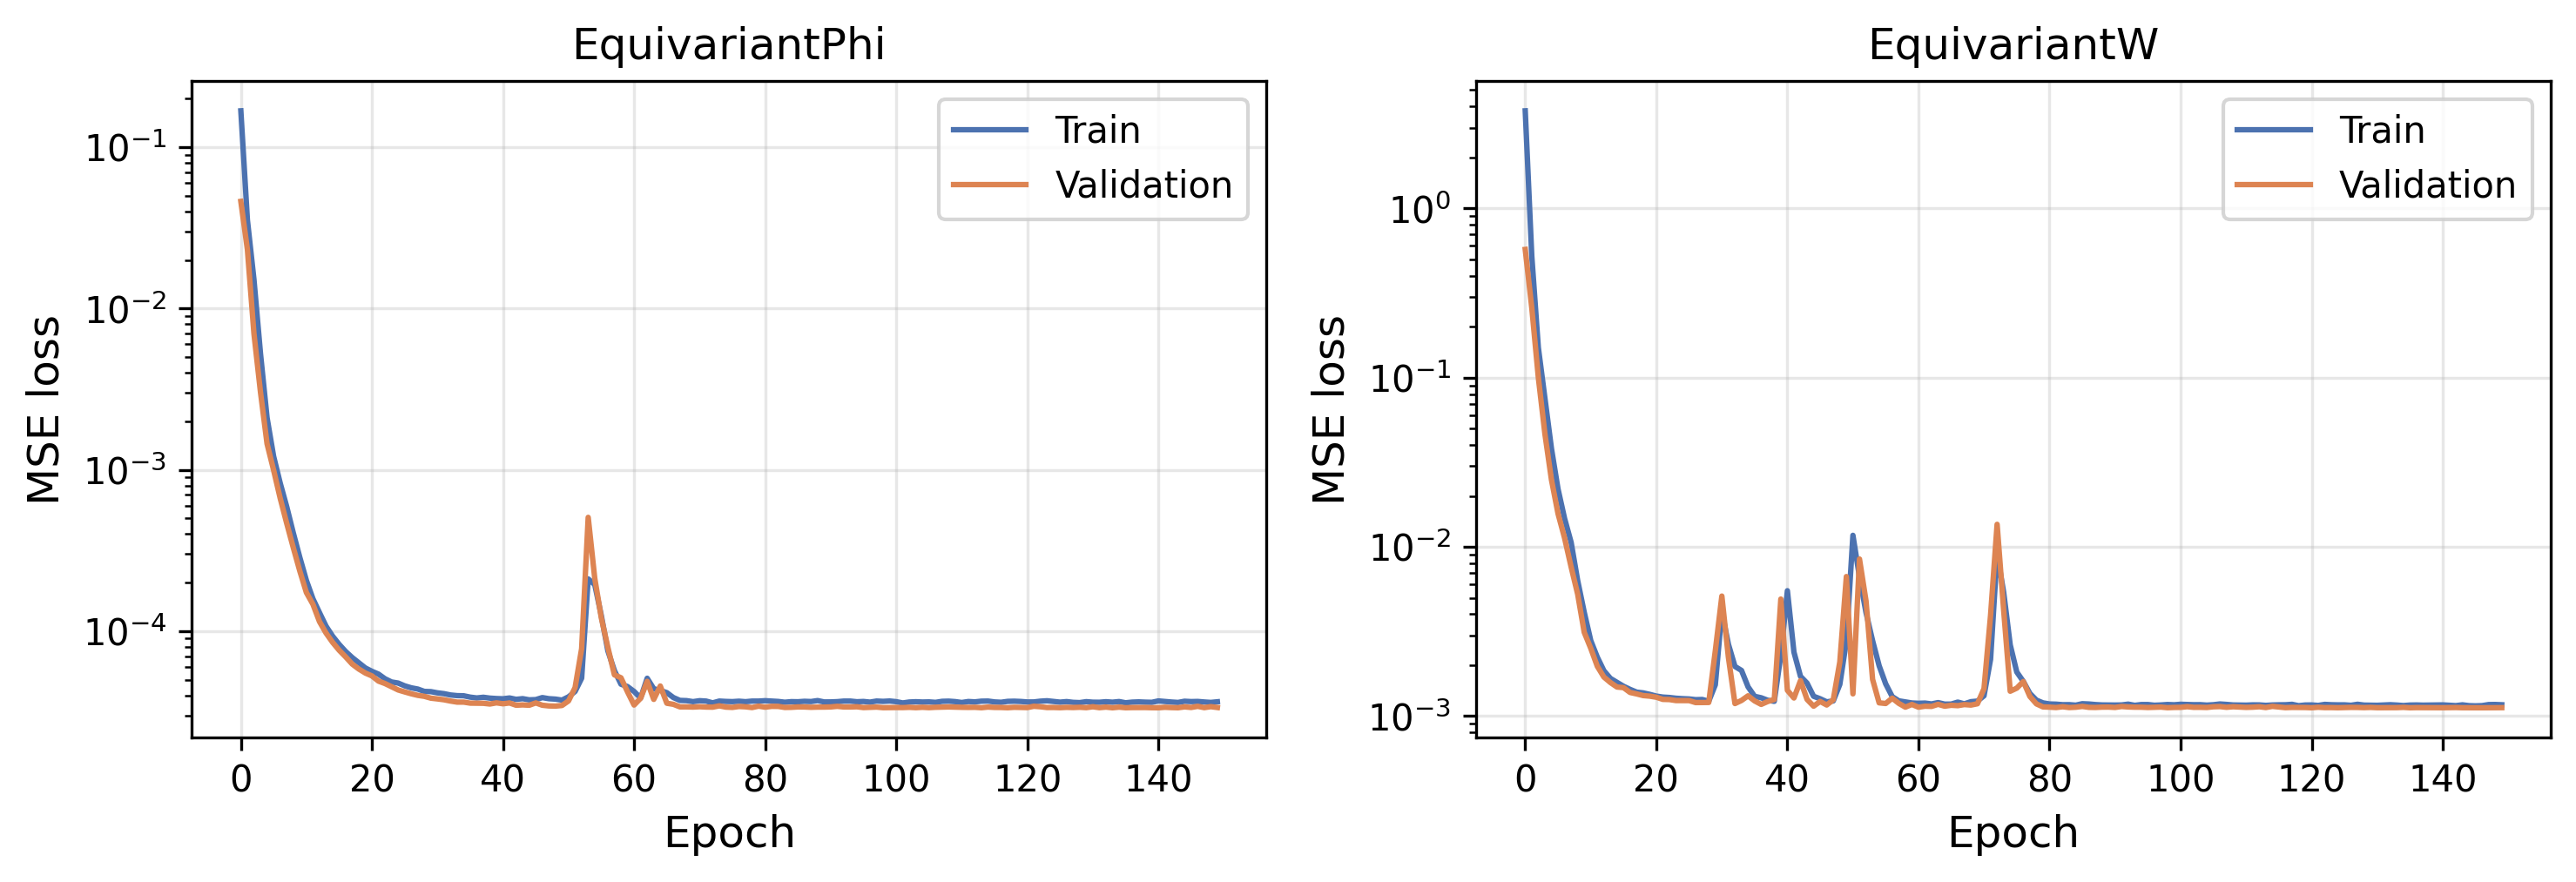
\includegraphics[width=0.8\textwidth]{../figures/thy_q3_training.png}
    \caption{Training curves for EquivariantPhi and EquivariantW.}
    \label{fig:q3_training}
\end{figure}

\textbf{Verification of exact equivariance.}
Repeating the tests from Sections~1--2, the Lorentz equivariance errors
are now of order $10^{-7}$ (Table~\ref{tab:q3_equivariance}), consistent
with float32 precision and representing an improvement of five to six
orders of magnitude over the original networks.

\begin{table}[htbp]
    \centering
    \caption{Lorentz equivariance errors: original vs equivariant architectures.}
    \label{tab:q3_equivariance}
    \begin{tabular}{cccc}
    Model & Transformation & Original & Equivariant \\
    \hline
    $\Phi$ & SO(3) rotation & 0.0562 & 1.99e-07 \\
    $\Phi$ & Lorentz boost & 0.0416 & 2.60e-07 \\
    $W$ & SO(3) rotation & 0.2302 & 3.45e-07 \\
    $W$ & Lorentz boost & 0.1415 & 4.80e-07
    \end{tabular}
\end{table}

\textbf{Emulation quality.}
On the validation set, EquivariantPhi achieves a mean relative error of
5.3\% (median 3.5\%), while EquivariantW gives 30.9\% (median 15.7\%).
The higher error for $W$ is expected: Equation~\eqref{eq:eq_W} is the
most general exactly equivariant form, but NN2 is only approximately
equivariant, so its non-equivariant components cannot be captured and a
residual error is unavoidable.

\section{Q4: Invariant Lagrangian Construction}

\subsection*{Analytic form}
\mbox{}\\
We construct a classical Lagrangian with kinetic and mass terms for both
fields:
%
\begin{equation}\label{eq:lagrangian}
\mathcal{L} = \partial_\mu \Phi^\dagger \partial^\mu \Phi
            - m_\Phi^2\,\Phi^\dagger \Phi
            - \tfrac{1}{4}\,G_{\mu\nu}^a\,G^{\mu\nu\,a}
            + \tfrac{1}{2}\,m_W^2\,W_\mu^a\,W^{\mu\,a},
\end{equation}
%
where $G_{\mu\nu}^a = \partial_\mu W_\nu^a - \partial_\nu W_\mu^a$ is the
Abelian field-strength tensor. We omit the non-Abelian
$g\epsilon^{abc}W_\mu^b W_\nu^c$ self-interaction since we work with a
global (not gauged) SU(2) symmetry and the Abelian kinetic term already
demonstrates the required invariance structure.

\textbf{Lorentz invariance.}
Every Lorentz index is contracted: $\partial_\mu\Phi^\dagger\partial^\mu\Phi$
contracts two vector indices via $\eta^{\mu\nu}$; $G_{\mu\nu}^a G^{\mu\nu\,a}$
contracts two antisymmetric tensor pairs; and $W_\mu^a W^{\mu\,a}$ contracts
one pair. Since $\Phi$ is a scalar and $W_\mu^a$ a vector, each term is a
Lorentz scalar.

\textbf{SU(2) invariance.}
$\Phi^\dagger\Phi$ is invariant under $\Phi \to U\Phi$ by unitarity.
All adjoint indices $a$ are contracted with $\delta^{ab}$, preserved under
$W^a \to R^{ab}W^b$ by orthogonality of $R$.

\subsection*{Implementation and results}
\mbox{}\\
The equivariant networks output $W^{\mu}_a$ with an upper Lorentz index;
we lower with $W_\nu^a = \eta_{\nu\mu}\,W^{\mu}_a$ before forming
$G_{\mu\nu}^a$. All derivatives are computed exactly via PyTorch autograd.
To ensure well-defined second derivatives we retrain with SiLU activations
in place of ReLU, achieving comparable emulation quality
(Figure~\ref{fig:q4_training}). We set $m_\Phi = m_W = 1$.

\begin{figure}[htbp]
    \centering
    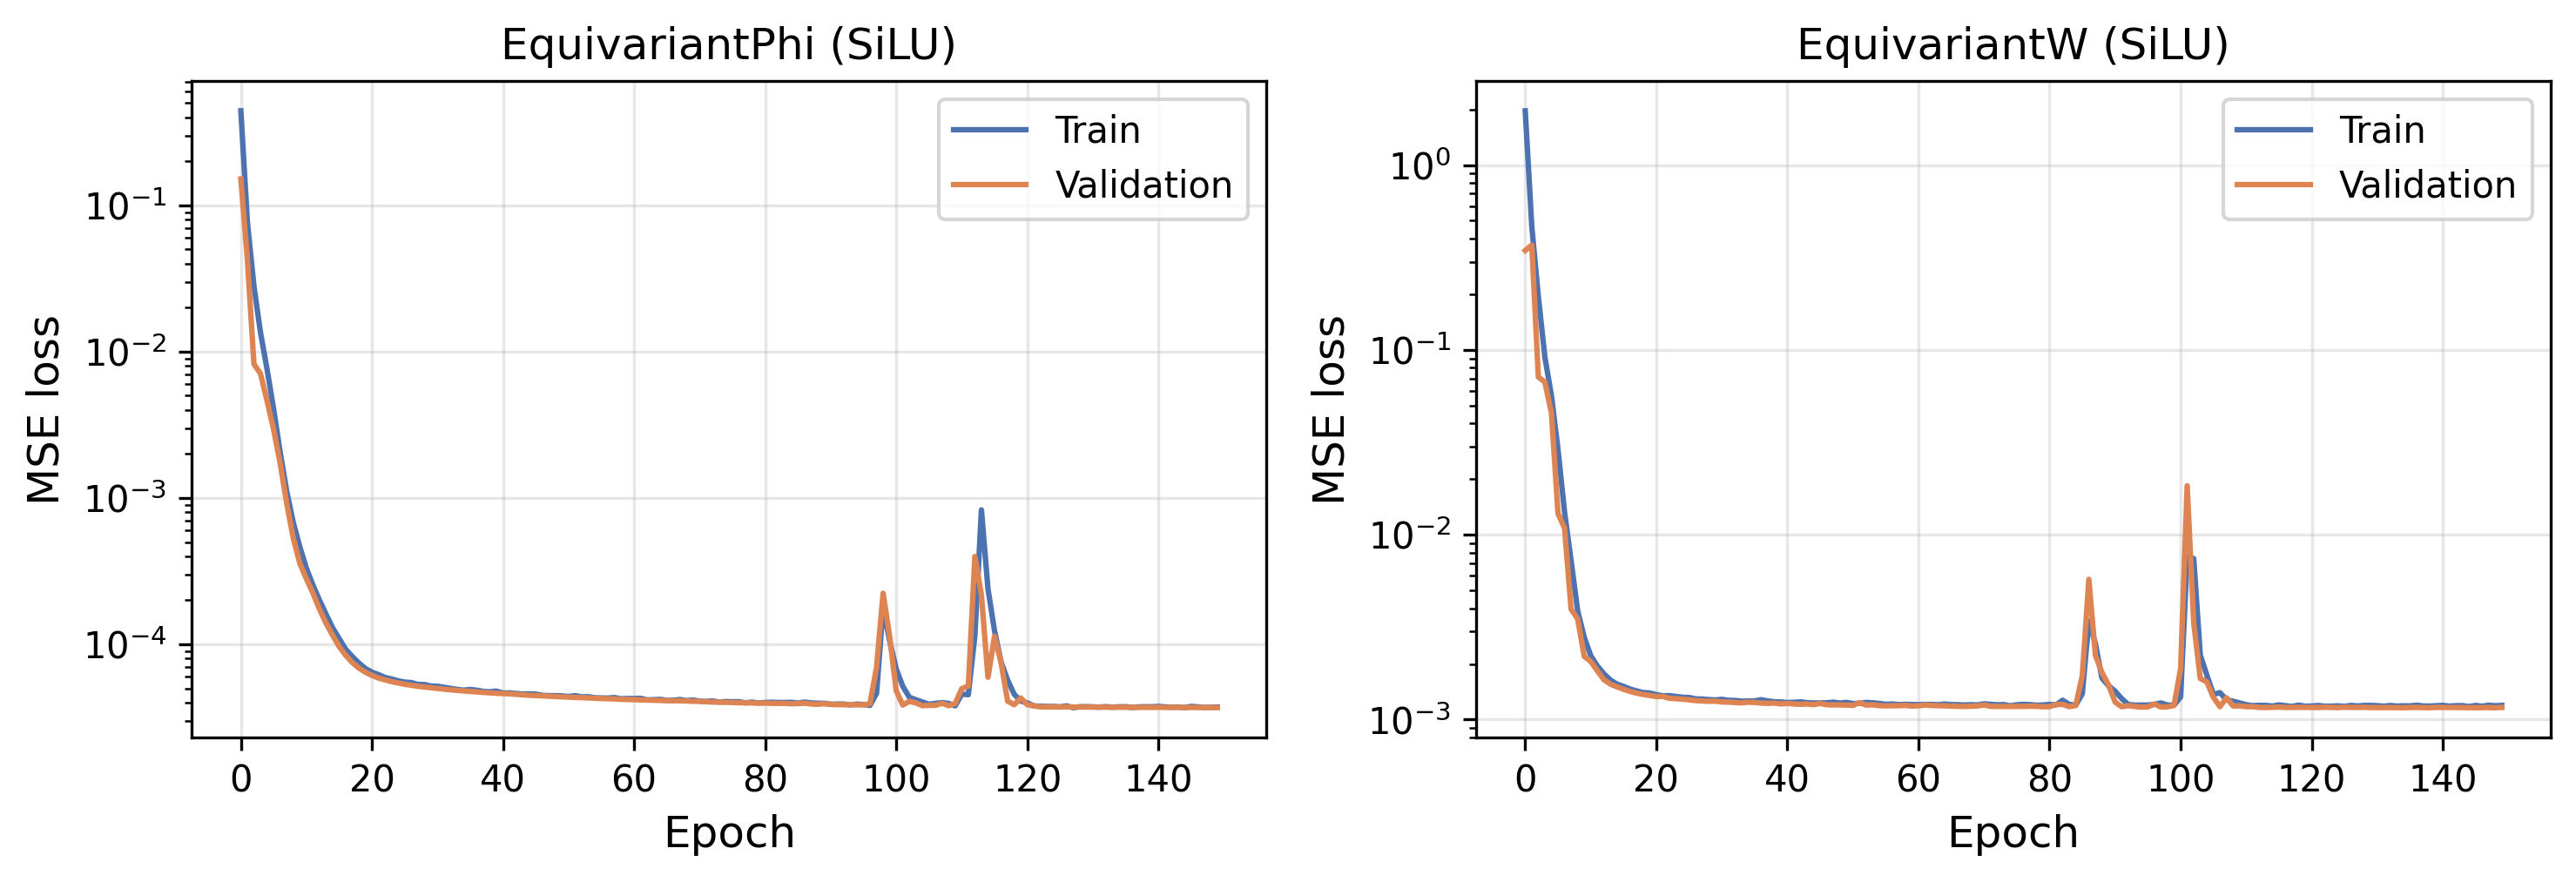
\includegraphics[width=0.8\textwidth]{../figures/thy_q4_training.png}
    \caption{Training curves for SiLU equivariant networks.}
    \label{fig:q4_training}
\end{figure}

\textbf{Lorentz invariance (numerical).}
We evaluate $\mathcal{L}(x)$ and $\mathcal{L}(\Lambda x)$ at 15 random
points under random SO(3) rotations and Lorentz boosts. The mean relative
errors are $1.7 \times 10^{-7}$ and $2.7 \times 10^{-7}$ respectively, 
confirming that the Lagrangian is a Lorentz scalar to machine precision.

\textbf{SU(2) invariance (numerical).}
Under random $U \in \mathrm{SU}(2)$, the maximum deviations in
$\Phi^\dagger\Phi$ and $W_\mu^a\,W^{\mu\,a}$ are
$4.7 \times 10^{-8}$ and $2.3 \times 10^{-7}$ respectively, consistent
with float32 precision. This follows because the Lagrangian depends on
the fields only through unitarily invariant ($\Phi^\dagger\Phi$) and
orthogonally invariant ($\delta_{ab}$) contractions.

\section*{Use of generative AI}
Claude (Anthropic) was used to assist with code development and
report writing. All outputs were reviewed and tested by the author,
who takes full responsibility for the final submission.

% \begin{thebibliography}{99}

% \bibitem{1} ***

% \end{thebibliography}
\end{document}